% !TEX TS-program = pdflatex
% !TEX encoding = UTF-8 Unicode
% arara: pdflatex: { synctex: true, shell: true }
\pdfminorversion=7
\documentclass[t]{beamer}
\usetheme{texsx}
\usepackage[czech]{babel}	
\usepackage{lmodern}
\usepackage[T1]{fontenc}
\usepackage[utf8]{inputenc}
\usepackage{subcaption}
\usepackage{media9}

\DeclareMathOperator{\sgn}{sgn}
\DeclareMathOperator*{\argmax}{argmax}
\DeclareMathOperator*{\softmax}{softmax}
\DeclareMathOperator*{\argsoftmax}{argsoftmax}
\DeclareMathOperator*{\argmin}{argmin}
\DeclareMathOperator{\atan2}{atan2}
\newcommand{\norm}[1]{\lVert #1 \rVert}



\title{Deep Closest Point}
\author{Nikolay Tsoy, Vojtěch Nydrle}
\markboth{VIR, leden 2020}{}
\date{\today}

\addtobeamertemplate{navigation symbols}{}{%
    \usebeamerfont{footline}%
    \usebeamercolor[fg]{footline}%
    \hspace{1em}%
    \insertframenumber/\inserttotalframenumber
}
  
  
\begin{document}

\begin{frame}
	\thispagestyle{empty}
  \titlepage
  %\frametitle{Title}
  %\tableofcontents[currentsection]
\end{frame}

    
\begin{frame}<beamer>
  \frametitle{Zadání}
	\onslide<2->\textbf{Tema OJ1:}
  \begin{itemize}
\onslide<2-> \item Vyzkoušet DCP (https://arxiv.org/abs/1905.03304) na real-world datech jako náhrada standardního SLAM algoritmu.
  \end{itemize}
  
  
  \onslide<3->\textbf{DCP}
    \begin{itemize}
\onslide<3-> \item Deep Closest Point
\onslide<3-> \item Deep Learning náhrada ICP
  \end{itemize}  
\end{frame}


\begin{frame}<beamer>
  \frametitle{ICP}
	\onslide<2->\textbf{Iterační algoritmus}
  \begin{itemize}
	\onslide<3-> \item určuje $\textbf{R}_{xy}$ a $\vec{t}_{xy}$ mezi množinami bodů $X$ a $Y$
	\begin{itemize}
  		\onslide<3-> \item $X=\lbrace \vec x_1, \ldots, \vec x_N \rbrace \subset \mathbb{R}^3$
  		\onslide<3-> \item $Y=\lbrace \vec y_1, \ldots, \vec y_N \rbrace \subset \mathbb{R}^3$
  		\onslide<3-> \item $Y$ vznikne otočením a posunutím $X$
  \end{itemize}
  
  
  \onslide<4-> \item tak aby $E(\textbf{R}_{xy},\vec{t}_{xy})$ byla minimální
	\begin{itemize}
  		\onslide<4-> \item $\displaystyle E(\textbf{R}_{xy},\vec{t}_{xy})=\frac{1}{N}\sum_{i=1}^N \norm{\textbf{R}_{xy}\vec x_i+\vec{t}_{xy} -\vec y_{m(x_i)}}^2 $
  		
  		
  		\onslide<4-> \item $\displaystyle m(x_i)=\argmin_j \norm{\textbf{R}_{xy}\vec x_i+\vec{t}_{xy} -\vec y_j}^2 $
  \end{itemize}
  \end{itemize}  
\end{frame}


\begin{frame}<beamer>
  \frametitle{Problémy ICP}
	%\onslide<2->\textbf{Iterační algoritmus}
  \begin{enumerate}
  \onslide<2-> \item nelze optimalizovat  $\textbf{R}_{xy}$, $\vec{t}_{xy}$ i $m$ najednou
  \onslide<3-> \item v jednom kroku optimalizuje $m$ a v dalším  $\textbf{R}_{xy}$ a $\vec{t}_{xy}$
  \onslide<4-> \item velmi často najde jen lokální optimum
  \onslide<5-> \item neuvažuje zajímavost některých bodů 
  \onslide<6-> \item neporadí si se šumem a řídkostí měření 
  \end{enumerate}  
\end{frame}



\begin{frame}<beamer>
  \frametitle{DCP}
  \begin{enumerate}
  \onslide<2-> \item nejprve stanoví $m(x_i)$ 
  \onslide<3-> \item z odpovídajících si $\vec x_i$ a $\vec y_i \in \mathbb{R}^3$ vypočte $\textbf{R}_{xy}$ a $\vec{t}_{xy}$
  \onslide<4-> \item $\displaystyle \vec x_c = \frac{1}{N}\sum_{i=1}^N\vec x_i,~\vec y_c = \frac{1}{N}\sum_{i=1}^N\vec y_i$
  \onslide<5-> \item $\displaystyle \textbf{H} = \sum_{i=1}^N (\vec x_i-\vec x_c)(\vec y_{m(x_i)}-\vec y_c)^T = \textbf{USV}^T$
  \onslide<6-> \item $\displaystyle \textbf{R}_{xy}=\textbf{VU}^T, ~ \vec{t}_{xy}=\vec y_c - \textbf{R}_{xy}\vec x_c$
  \end{enumerate}  
\end{frame}


\begin{frame}<beamer>
  \frametitle{DCP - nalezení $m(x_i)$}
  \begin{enumerate}
  \onslide<2-> \item PointNet nebo DGCNN před poslední vrstvou 
  \onslide<3-> \item generuje $\textit{F}_X=\lbrace \vec x_1^L, \ldots, \vec x_N^L  \rbrace \subset \mathbb{R}^P $ a $\textit{F}_Y=\lbrace \vec y_1^L, \ldots, \vec y_N^L  \rbrace \subset \mathbb{R}^P$
  \onslide<4-> \item $\vec x_i^L$ a $\vec y_i^L$ "sémanticky" popisují bod $\vec x_i$ a $\vec y_i$
  \onslide<5-> \item $\displaystyle m(x_i)=\softmax(\Phi(Y)^T {\Phi(x_i)})$, $\Phi$ je "Transformer"
  \onslide<6-> \item taky poznáváme podobné body ne podle barvy a polohy ale podle významu
  \end{enumerate}  
\end{frame}


\begin{frame}<beamer>
  \frametitle{DCP}
  \onslide<2->\textbf{Učení:}
  \begin{enumerate}
  \onslide<2-> \item $\displaystyle L=\norm{\textbf{R}_{xy}^T\textbf{R}_{xy}^g-I}^2 + \norm{\vec{t}_{xy}-\vec{t}_{xy}^g}^2+\lambda \norm{\theta}$
  \onslide<2-> \item $\textbf{R}_{xy}^g$ a $\vec{t}_{xy}^g$ popisují skutečnou transformaci, $\theta$ jsou parametry CNN
	\end{enumerate} 
	\onslide<3->\textbf{Závěr autorů:}
	\begin{enumerate}  
   \onslide<4-> \item DCP je dost spolehlivý na určení kvalitního výstupu v jednom běhu, ale nechá se ještě doplnit ICP.
  \onslide<5-> \item Může být snadno použit ve složitějších například SALM
  \end{enumerate}  
\end{frame}


\begin{frame}<beamer>
  \frametitle{Naše práce}
  \onslide<2->\textbf{Dataset:}
  \begin{itemize}
 	\onslide<2-> \item "KITTI Vision"  22 sekvencí k 11 se skutečnou pozici
  \onslide<3-> \item na jedné sekvenci jsme učily a druhé testovaly
	\end{itemize} 
	\onslide<3->\textbf{Problémy začlenění KITTY do DCP:}
	\begin{enumerate}  
   \onslide<4-> \item celý lidarový záběr je natolik velký při forwardpass spotřebuje víc jak 16 GB RAM
    proto jsme použili jen prvních $N$ bodů
   \onslide<5-> \item špatně jsme pochopili popis datasetu a trénovaly na špatně spočítaných rotačních maticích
  \end{enumerate}  
\end{frame}

\begin{frame}<beamer>
  \frametitle{Dosažené výsledky}
%  \onslide<2->\textbf{Učení:}
  \begin{enumerate}
  \onslide<2-> \item načíst dataset do formátu, který vyžaduje DCP
	\onslide<3-> \item natrénovat na prvních $N$ bodech pointkloudů jedné sekvence \onslide<5-> na testovacích datech veliká chyba
  \onslide<6-> \item natrénovat na náhodných $N$ bodech pointkloudů jedné sekvence\onslide<7-> zlepšení výsledků
  \onslide<7-> \item předělat dataset na trénování všech kombinacích záběrů se společnou částí scény
  \onslide<8-> jedna epocha se trénuje přes dvě hodiny $\rightarrow$ nestihly jsme natrénovat
%  \onslide<6-> \item 
  \end{enumerate}  
\end{frame}

\begin{frame}<beamer>
  \frametitle{Dosažené výsledky}
\begin{figure}[htb]
		\begin{overprint}
		\centering
		\onslide<1> 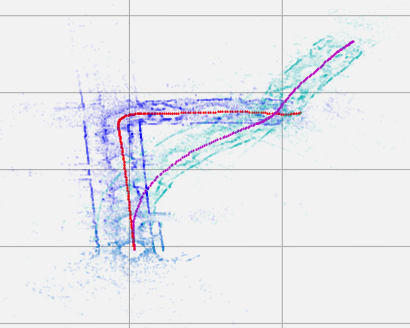
\includegraphics[width=0.6\textwidth]{02.png}
		\onslide<2> 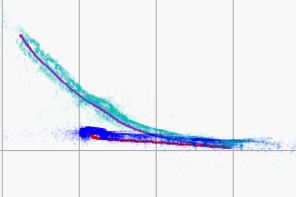
\includegraphics[width=0.6\textwidth]{01.png}
		%\onslide<3> \includegraphics[width=0.6\textwidth]{matrix-02.pdf}
		%\onslide<4> \includegraphics[width=0.6\textwidth]{matrix-03.pdf}
		\end{overprint}
\end{figure}
\end{frame}

\begin{frame}<beamer>
  \frametitle{Proč to nefunguje?}
%  \onslide<2->\textbf{Učení:}
  \begin{enumerate}
  \onslide<2-> \item testováno na otočený, posunutých a zašuměných objektech
	\onslide<3-> \item ne na deformovaných objektech
  \onslide<6-> \item přebývající body jsou špatně přiřazeny
  \end{enumerate} 
  \onslide<7->\textbf{Lze to zpravit?}
  \begin{enumerate}
  \onslide<8-> \item záběru odstranit část scény (určenou směrem a rychlostí pohybu)
  \onslide<9-> \item hypotézu lze ověřit otestováním na datech z interiéru
  \end{enumerate}  
\end{frame}


\begin{frame}<beamer>
  \frametitle{Možné zlepšení}
\begin{itemize}
\onslide<2-> \item Nahradit $m=\softmax(\Phi_Y(y)^T \Phi_X(x_i))$ složitější funkcí, která by se nesnažila přiřadit body co nejsou v druhé množině.
\onslide<3-> \item Trénovat neuronovou sít na více jízdách než jen na jedné.
\onslide<4-> \item Při výpočtu aktuální pozice nevycházet jen z předešlého záběru scény ale všech v dosahu lidaru.
\onslide<5-> \item Po vypočtení pozice pomocí DCP použít na tento výsledek ještě ICP pro zpřesnění výsledku.
\end{itemize}
\end{frame}




		




\begin{frame}<beamer>
  \frametitle{Děkujeme za pozornost}
  
 %\includemedia[
%     width=6cm,height=6cm,
%     activate=pageopen,
%     addresource=LPE2.mp4,
%     flashvars={
%         source=LPE2.mp4
%        &autoPlay=true
%     }
%]{}{VPlayer.swf}
\end{frame}		

\end{document}
